\bookchapter{Глава 60. Настраиваем среду разработки — Xcode и первый проект}

\chapterintro{Чтобы дело спорилось, сначала нужно наточить инструменты. В этой главе мы обустроим «кухню»: установим Xcode, запустим симулятор, создадим первый в жизни проект iOS и разберём структуру проекта по косточкам. Когда среда будет готова, вы впервые увидите, как написанный вами код превращается в кнопку, которую можно нажать, — этот момент многие запоминают на всю жизнь.}

\booksection{Готовим Mac}

Сначала о барьере: разработка под iOS возможна только на macOS. Если у вас нет Mac, есть три варианта: купить (подойдёт даже б/у Mac mini или MacBook Air), на короткий срок арендовать облачный Mac или сначала прочитать часть 8 «Практика разработки под Android» (там хватит и Windows).

\begin{center}
\begin{tabularx}{\linewidth}{|X|X|X|}
\hline
\textbf{Параметр} & \textbf{Минимум} & \textbf{Комфортный уровень (рекомендуется)} \tabularnewline
\hline
Чип & Apple Silicon (от M1) & M2 и новее \tabularnewline
Память & 8GB & 16GB \tabularnewline
Диск & Запас от 40 ГБ+ (сам Xcode весьма «упитанный») & от 256 ГБ \tabularnewline
Система & новейшая macOS & держать автообновление включённым \tabularnewline
\hline
\end{tabularx}
\end{center}

\begin{center}\small\color{gray}Ориентировочная конфигурация Mac для разработки (август 2026 года)\end{center}

\begin{tcbinfo}{Совет: без Mac язык тоже можно начать учить}
Бесплатное приложение Swift Playgrounds на iPad поможет освоить основы Swift (Mac не нужен); оно ставится даже на iPhone. Освойте в Playgrounds языковой материал главы 61, а когда появится Mac — сразу взлетите. Недаром говорят: хорошо наточенный топор дров не портит.

\end{tcbinfo}

\booksection{Устанавливаем Xcode}

Xcode — официальная интегрированная среда разработки Apple, бесплатная. Установка в три шага:

\begin{enumerate}
  \item Откройте на Mac App Store, найдите «Xcode» и нажмите «Установить» — учтите, он весит несколько гигабайт, выберите время с хорошей скоростью сети;
  \item При первом запуске после установки примите лицензионное соглашение и дождитесь установки компонентов (происходит автоматически);
  \item В меню Xcode Settings Locations убедитесь, что выбран Command Line Tools — инструменты командной строки нужны многим скриптам и сторонним инструментам.
\end{enumerate}

\begin{tcbwarn}{Внимание: «игра в соответствие» версий и системы}
Новый Xcode обычно требует новейшую macOS, а старый Mac может застрять на старой версии. При публикации в App Store Apple требует собирать приложение более свежим Xcode (обычно давая отсрочку). Поэтому не затягивайте с обновлением системы — iOS-разработчики самые усердные «охотники за новыми версиями».

\end{tcbwarn}

\booksection{Создаём ваш первый проект}

Откройте Xcode Create New Project выберите iOS шаблон App, затем заполните:

\begin{center}
\begin{tabularx}{\linewidth}{|X|X|X|}
\hline
\textbf{Параметр} & \textbf{Что вводить} & \textbf{Пояснение} \tabularnewline
\hline
Product Name & MyFirstApp & Название приложения \tabularnewline
Team & ваш Apple ID (бесплатно) & нужен для подписи, личного аккаунта достаточно \tabularnewline
Organization Identifier & com.example & вместе с Product Name образует идентификатор пакета \tabularnewline
Interface & SwiftUI & основной фреймворк этой книги \tabularnewline
Language & Swift & без комментариев \tabularnewline
\hline
\end{tabularx}
\end{center}

\begin{center}\small\color{gray}Пять вещей, которые заполняются при создании проекта\end{center}

После нажатия Create Xcode сгенерирует проект, который можно запустить сразу. В левом верхнем углу выберите симулятор (например, iPhone 17) и нажмите > — через несколько секунд на экране симулятора появится окно с надписью «Hello, world!». Ваше первое приложение iOS родилось.

\booksection{Разбираем структуру проекта: зачем нужен каждый файл}

Слева находится навигатор проекта; новичку достаточно знать лишь несколько пунктов:

\begin{center}
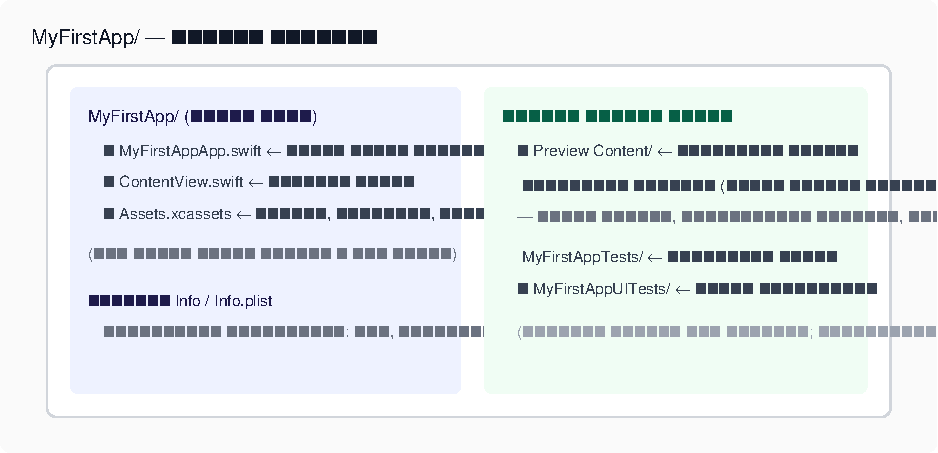
\includegraphics[width=0.92\linewidth]{figures/fig-di-liu-shi-zhang-1}
\\[2pt]\small Рисунок 2. Структура проекта Xcode, которую обязан понять новичок
\end{center}

\begin{itemize}
  \item MyFirstAppApp.swift: точка входа программы; в SwiftUI она занимает всего несколько строк — «запусти, затем покажи главный экран»;
  \item ContentView.swift: главное представление экрана; всё, что вы сейчас видите, находится здесь;
  \item Assets.xcassets: хранилище ресурсов — сюда кладут иконки, картинки и цвета;
  \item Настройки Target: нажмите на синий значок проекта слева — внутри номер версии, минимальная версия iOS и подпись. Здесь же настраиваются отображаемое имя и иконка приложения.
\end{itemize}

\booksection{Отладка на реальном устройстве: устанавливаем приложение на ваш iPhone}

\booksection{Приёмы эффективности в Xcode: пять «читов» с горячими клавишами для новичка}

Освоив эти приёмы, вы будете выглядеть «очень профессионально»:

\begin{center}
\begin{tabularx}{\linewidth}{|X|X|X|}
\hline
\textbf{Действие} & \textbf{Горячая клавиша} & \textbf{Назначение} \tabularnewline
\hline
Запуск & CmdR & Скомпилировать и запустить \tabularnewline
Открыть/переключить предпросмотр на холсте & OptionCmd & Переключатель «что видишь, то и получаешь» \tabularnewline
Форматирование отступов & CtrlI & Автоматически выровнять отступы выделенного кода \tabularnewline
Быстрое открытие файла & CmdO & Введите имя файла — откроется мгновенно (самое ходовое!) \tabularnewline
Закомментировать/раскомментировать & Cmd/ & Быстро включать/выключать код во время отладки \tabularnewline
\hline
\end{tabularx}
\end{center}

\begin{center}\small\color{gray}Частые горячие клавиши Xcode (пятёрка новичка)\end{center}

Ещё два скрытых бонуса: несколько симуляторов сразу (запустить iPhone и iPad одновременно и сравнить компоновку) и библиотека фрагментов кода (перетащите часто используемые строки в панель Snippets справа — в следующий раз вставите одним нажатием). Начните пользоваться инструментами эффективности — и ловкость придёт сама.

\booksection{Отладка на реальном устройстве: устанавливаем приложение на ваш iPhone}

Симулятор хорош, но финиш — на реальном устройстве. Отлаживать на нём можно и с бесплатным Apple ID:

\begin{enumerate}
  \item Соедините iPhone кабелем (или отлаживайте по Wi-Fi в одной сети);
  \item В списке устройств вверху Xcode выберите свой телефон; при первом подключении появится предложение войти в Apple ID, и подпись настроится автоматически;
  \item На iPhone: [Настройки] [Основные] [VPN и управление устройствами] доверьтесь сертификату вашего разработчика;
  \item Нажмите > — приложение установится на реальное устройство.
\end{enumerate}

\begin{tcbwarn}{Внимание: «семидневное ограничение» бесплатного аккаунта}
Приложение, подписанное бесплатным Apple ID, перестанет работать через 7 дней (чтобы продлить, просто запустите его ещё раз). Это защитный механизм Apple; на этапе обучения его вполне хватает, а у платного аккаунта разработчика (99 долларов в год) такого ограничения нет — подробнее в главе 67.

\end{tcbwarn}

\booksection{Первые пробы + скорая помощь при частых ошибках}

\booksection{Первые пробы + скорая помощь при частых ошибках}

Откройте ContentView.swift, замените текст в Text(“Hello, world!”) на своё имя и нажмите CmdR для повторного запуска — через несколько секунд на симуляторе появится ваше имя. Поздравляем: вы прошли свой первый полный цикл «изменил код скомпилировал установил запустил».

\begin{center}
\begin{tabularx}{\linewidth}{|X|X|X|}
\hline
\textbf{Симптом ошибки} & \textbf{Частая причина} & \textbf{Лекарство} \tabularnewline
\hline
Ошибка Signing & не выбран Team, истёк срок сертификата & в Target Signing отметьте свой аккаунт; с бесплатным аккаунтом запустите ещё раз \tabularnewline
Симулятор с чёрным экраном / не запускается & повреждённый образ & меню Device Erase All Content; либо удалите симулятор и создайте заново \tabularnewline
Xcode медленно скачивается / не устанавливается & скачки сети в App Store & попробуйте в другое время; или скачайте офлайн-пакет .xip с сайта разработчиков Apple \tabularnewline
\hline
\end{tabularx}
\end{center}

\begin{center}\small\color{gray}Таблица скорой помощи при ошибках окружения у новичков\end{center}

\begin{tcbpractice}{Попробуйте сами: пройдите свой «обряд посвящения» в разработчики}
(1) установите Xcode и запустите симулятор; (2) запустите своё приложение на реальном устройстве и сделайте памятный скриншот; (3) замените текст Hello на своё имя; (4) в настройках Target смените отображаемое имя приложения на «Моё первое приложение». Сделав эти четыре шага, вы становитесь автором собственного приложения.

\end{tcbpractice}

\begin{tcbsummary}{Краткие итоги главы}
\begin{itemize}
  \item Жёсткий барьер: Mac + Xcode; нет Mac — начните учить язык в Swift Playgrounds на iPad
  \item Xcode ставится из App Store; новая версия требует новую систему — не затягивайте с обновлениями
  \item Пять элементов нового проекта: имя, Team, идентификатор организации, SwiftUI, Swift
  \item Мантра проекта: весь код — в каталоге MyFirstApp/; настройки Target отвечают за версию и подпись
  \item При отладке на устройстве с бесплатным Apple ID подпись действует 7 дней; у платного аккаунта этого ограничения нет
  \item Быт разработчика = изменить код CmdR посмотреть результат, и так по кругу
\end{itemize}

\end{tcbsummary}
